\documentclass[../../Atom-ogMolekylefysik.tex]{subfiles}
\begin{document}
\section{Molekylefysik}
Vi har hidtil ignoreret orbitalernes rummelige form. For isolerede atomer er det nemlig ikke super vigtigt. For molekyler er det derimod essentielt, og der er vidst nogle eksempler på figur \ref{fig:orbitalform}. De simpleste orbitaler er $s$ orbitalerne. De er sfærisk symmetriske. Normalt repræsenteres de som en kugle, der angiver det område, hvor det er mest sandsynligt at finde elektronen.
Hvor $s$ orbitalerne var de eneste med deres bestemte energi, kommer $p$ orbitalerne i sæt af tre. Her er der størst sandsynlighed for at finde elektronen i to regioner på hver sin side af atomkernen. Selve bølgefunktionen har hvert sit fortegn i disse regioner. Orbitalerne ligger langs en akse, og normalt navngives de derfor: $p_x$, $p_y$ og $p_z$. De repræsenteres oftest som en ottetalsformet overflade med to forskellige farver til at angive fortegnet.
\begin{figure}[h!]
    \centering
    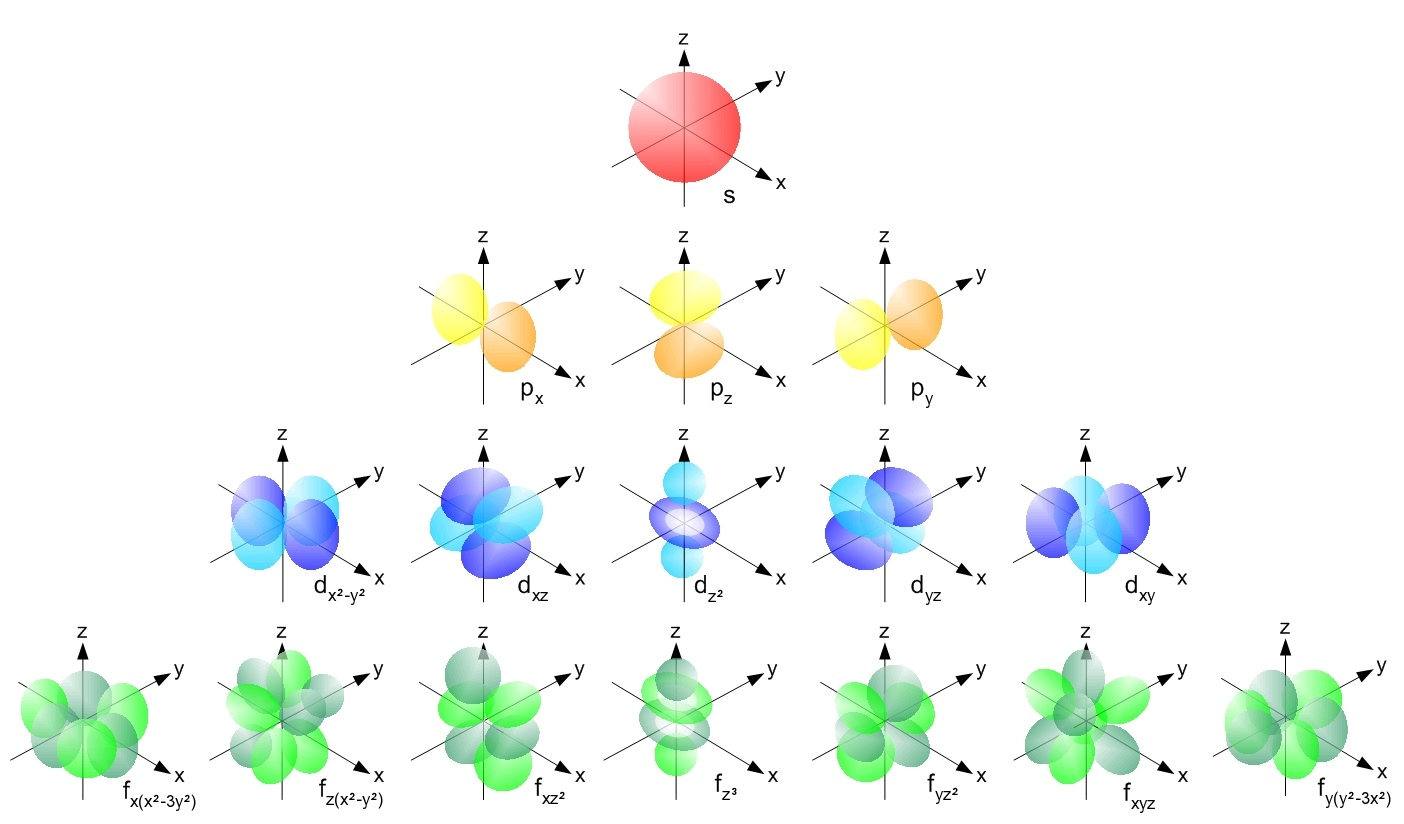
\includegraphics[width = \textwidth]{Atom-ogMolekylefysik/billeder/Single_electron_orbitals.jpg}
    \caption{Formen på $s$, $p$, $d$ og $f$ orbitalerne. Bemærk at indekserne er tre dimensionelle polynomier, som har samme symmetri som orbitalen. Kilde: Wikkimedia commons.}
    \label{fig:orbitalform}
\end{figure}
\subsection{LCAO}
Når to eller flere atomer bringes tæt på hinanden, vil deres elektroner interagere. Hvis det resulterende system er stabilt vil der dannes et molekyle. I et kovalent bundet molekyle er nogle af elektronerne ikke længere bundet til et atom, men delt imellem flere. Disse molekylære orbitaler kan dannes, som en sum af atomorbitaler. Denne metode kaldes LCAO metoden\footnote{LCAO står for Linear Combination of Atomic Orbitals, eller på dansk: LinearKombination af AtomOrbitaler.}.
Når to $s$ orbitaler blandes dannes to kombinationer: en bindende $\sigma$ orbital eller en antibindende $\sigma^*$ orbital. Den bindende orbital dannes ved at lægge $s$ orbitalerne sammen. Her vil der være en større sandsynlighed for at finde elektronen imellem atomkernerne, så elektronen tiltrækker kernerne stærkere end de frastøder hinanden. Det er dette der holder molekylet sammen.
For den antibindende orbital trækkes atomorbitalerne fra hinanden. Der vil derfor være en lavere sandsynlighed for at finde elektronen imellem kernerne, der derfor frastøder hinanden.
\begin{figure}[h!]
    \centering
    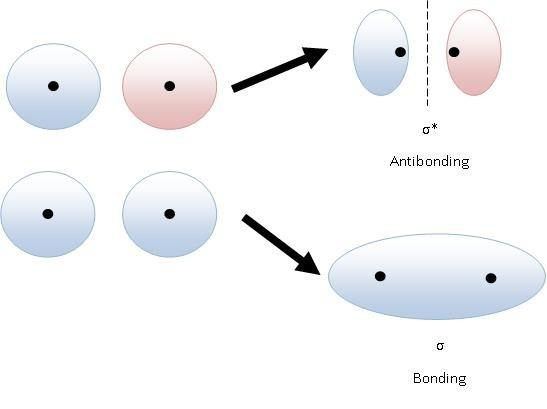
\includegraphics[width = 0.6\textwidth]{Atom-ogMolekylefysik/billeder/sigmaOrbital.jpg}
    \caption{Dannelsen af en bindende $\sigma$ og en antibindende $\sigma^*$ orbital.
    Kilde: \url{chemwiki.ucdavis.edu}}
    \label{fig:sigmaOrbital}
\end{figure}
Ser vi på et brintmolekyle H$_2$ som eksempel, ses det, at de indgåede atomer her har en $s$ orbital der indgår i bindingen. Brintmolekylet har derfor en bindnde og en antibindende orbital.
Molekylet indeholder i alt to elektroner. Der er plads til begge elektroner i den bindende orbital, så i grundtilstanden vil de begge være der. En let måde at tjekke, om et molekyle er stabilt, er at tælle antallet af fyldte bindende orbitaler, minus antallet af fyldte antibindende orbitaler. Dette tal kaldes molekylets bindingsorden. Er bindingsordenen større end nul vil, der være en energigevinst for atomerne ved at være i molekylet. Ellers kan molekylet ikke eksistere. Brintmolekylet har en fyldt bindende orbital, så bindingsordenen er 1. Molekylet er derfor stabilt. Dette passer med hvad vi ser i virkeligheden, hvor H$_2$ er et stabilt molekyle\footnote{Der dog er ret reaktivt.}. De to forskellige orbitaler for H$_2$ er vist på figur \ref{fig:sigmaOrbital}.  

\begin{figure}[h!]
    \centering
    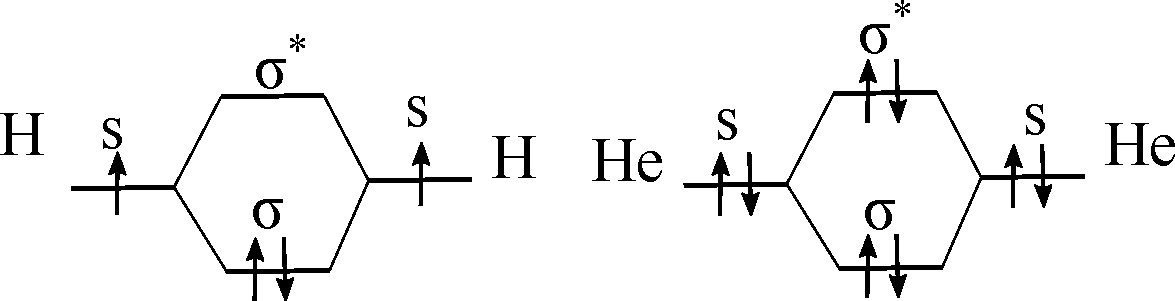
\includegraphics[width = \textwidth]{Atom-ogMolekylefysik/billeder/simpeltMOD.pdf}
    \caption{Diagram over orbitalerne i brintmolekylet og i dihelium. Pilene angiver elektronernes spin.}
    \label{fig:simpeltMOD}
\end{figure}

Nu er vi i stedet på et molekyle bestående af to helium atomer. Her indgår de samme orbitaler, men både den bindende og den antibindende orbital er fyldt. Bindingsordenen er derfor nul. Ganske rigtigt findes dihelium ikke i virkeligheden, og helium er {\em meget} uvillig til at reagere\footnote{Helium indgår i ingen kendte molekyler.}. Helt generelt vil stabile molekyler have høj bindingsorden.
\subsection{Binding med $p$ orbitaler}
Når bindingen involverer $p$ orbitalerne, er der lige pludseligt langt flere orbitaler involveret i bindingen. Ligesom for $s$ orbitalerne kan bindingen dannes langs bindingsaksen. Her vil de to $p$ orbitaler, der ligger langs aksen binde på samme måde som $s$ orbitalerne gjorde det. Her dannes igen et sæt af en $\sigma$ orbital og en $\sigma^*$ orbital. De resterende $p$ orbitaler indgår også i bindingen. De $p$ orbitaler der er vinkelrette på bindingsaksen vil også kunne overlappe. Her kaldes orbitalerne $\pi$ orbitaler. Der vil være to bindende $\pi$ orbitaler og to antibindende $\pi^*$ orbitaler, svarende til de fire $p$-orbitaler der indgår i dem. Overlappet imellem $p$-orbitalerne er mindre for $\pi$-bindingen end for $\sigma$-bindingen, så normalt er opsplitingen mindre her.

Vi kan opstille en række regler for hvordan atomorbitalerne blander, når molekylet binder.
\begin{enumerate}
    \item Atomorbitaler overlapper kun, når deres fortegn er det samme.\label{MODregelsym}
    \item Når to atomorbitaler blander dannes to molekylære orbitaler, en bindende og en antibindende.
    \item Hvis to orbitaler skal blande må de have omtrent samme energi.\label{MODregelenergi}
    \item Hver molekyleorbital kan indeholde to elektroner, en med spin i hver retning.
    \item Elektronstrukturen kan konstrueres ved at placere alle elektronerne med så lav en energi som muligt\footnote{Dette kaldes Aufbau princippet.}.
    \item Når flere orbitaler har samme energi placeres elektroner først enkeltvist, når alle de relevante orbitaler har en elektron, tilføjes elektron nummer to.
    \item Bindingsordenen af et diatomart molekyle er antallet af bindende elektronpar, minus antallet af antibindende elektronpar.
\end{enumerate}
Regel nummer \ref{MODregelsym} sørger for at $\sigma$ og $\pi$ orbitalerne ikke interagerer. Forskellige $\sigma$-orbitaler derimod er i princippet frie til at interagere. I de fleste tilfælde bliver vi redet af regel nummer \ref{MODregelenergi}. For de fleste atomer har $s$- og $p$-orbitalerne stor nok forskel i deres energi til, at det ikke giver mere end en mindre korrektion til det endelige billede. Da vi betragter problemet kvalitativt har det ingen betydning. Det vil dog have en betydning for diatomare molekyler med kvælstof(N) eller lettere grundstoffer\footnote{Det er grundstofferne: bor(B), kulstof(C) og kvælstof(N).}. Her ligger den bindende $\sigma$ orbital for $p$-orbitalerne højere i energi end den bindende $\pi$ orbital.
\begin{figure}[h!]
    \centering
    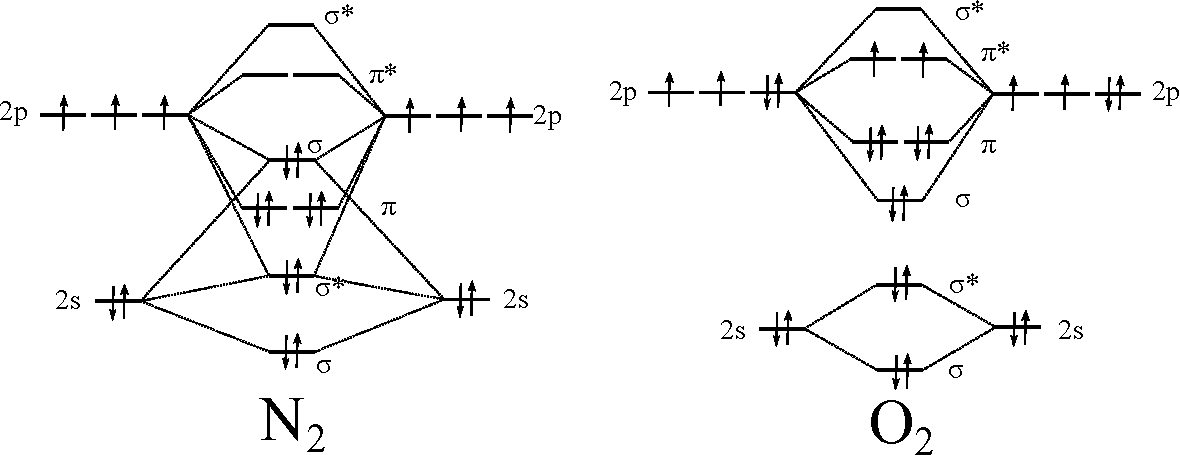
\includegraphics[width = \textwidth]{Atom-ogMolekylefysik/billeder/diatomarMOD.pdf}
    \caption{Molekyleorbitaldiagrammer for ilt og kvælstof molekyler. Bemærk ombytningen af $\pi$- og $\sigma$-orbitalerne i N$_2$.}
    \label{fig:diatomar}
\end{figure}

Er atomerne ikke de samme vil reglerne stadig gælde. Man skal blot huske at $s$-orbitaler giver $\sigma$ orbitaler, mens $p$ orbitaler giver både $\sigma$ orbitaler og dobbelt så mange $\pi$ orbitaler.

Vi behøver ikke at bekymre os om $d$- eller $f$-orbitaler. Når vi kommer så langt ned i det periodiske system, at de bliver relevante, vil alt være metaller, der sjældent binder kovalent med hinanden. Metalbinding er et helt andet emne, der på trods af at det er fascinerende, ligger uden for det vi vil dække her.

Tilsvarende regler gælder når man giver sig til at bygge større molekyler. Her er elektronerne nogle gange begrænset over et lille område af molekylet, men især $\pi$ bindinger har en tendens til at flyde sammen. I organiske molekyler så som benzen vil elektronerne ofte kunne bevæge sig frit over store dele af molekylet. 
\end{document}